\chapter[Källtexter --- Implicit notation]{Källtexter till Maple --- Implicit notation}
\label{FindImplicitNotation}

\section{FindImplicitNotation}

\emph{FindImplicitNotation}-funktionen beräknar den implicita notationen för en kurva, $C=\left\{(x,y)\in \mathbb{C}^2 : F(x,y)=0\right\}$ givet en explicit parametriserad version av samma kurva $C=C(\mathbb{R}), C(t)=(X_p(t),Y_p(t))$. För resultatet gäller att $F(X_p(t),Y_p(t))=0, \forall t \in \mathbb{R}$. Dessutom kommer $F(x,y)$ vara av minimal grad i den variabel som används för att definiera $X_p$ och $Y_p$. Funktionen tar också en maximal grad som används som övre gräns i sökalgoritmen, för att begränsa sökningen ifall resultat inte hittas.

\begin{table}[h]
\caption{Parametrar för \emph{FindImplicitNotation}}
\begin{center}
\begin{tabular}{|l|p{9cm}|}
\hline
$X_p$ & Parametriseringen av x-koordinaten. \\
$Y_p$ & Parametriseringen av y-koordinaten. \\
$Variable$ & Vilken variabel som använts vid parametriseringen.\\
$MaxDegree$ & Maximal grad vid sökning efter medlemmar i $\left<X_p , Y_p\right>$.\\
$PrintTime$ & En frivillig parameter. Om \emph{true} så skrivs tidsåtgången för beräkningen ut på skärmen.\\
\hline
\end{tabular}
\end{center}
\end{table}

\begin{verbatim}
FindImplicitNotation := proc(Xp, Yp, Variable, MaxDegree)
   local List, Pos, Count, ExpOrder, ExpOrders, MaxOrd, 
      Explicit, StartTime, CurrentMaxDegree, PrintTime, 
      Solution, i, j, k, f, g, p, x, y, a, b, c;

   StartTime := time();
   PrintTime := nargs < 5 or args[5];
   CurrentMaxDegree := MaxDegree;
   Solution := 0;
   f := Xp;
   g := Yp;

   if ldegree(f, Variable) = ldegree(g, Variable) then
      a := tcoeff(f, Variable);
      b := tcoeff(g, Variable);
      g := (g * a - f * b) / gcd(a,b)
   end if;

   List[0] := f;
   List[1] := g;
   Explicit[0] := x;
   Explicit[1] := y;
   MaxOrd := ldegree(f, Variable);
   ExpOrder[0] := MaxOrd;

   for i from 0 to MaxOrd - 1 do 
      ExpOrders[i] := -1 
   end do;

   ExpOrders[MaxOrd] := 0;
   j := ldegree(g, Variable);

   if MaxOrd < j then
      if MaxOrd + 1 < j then
         for i from MaxOrd + 1 to j - 1 do 
            ExpOrders[i] := -1 
         end do
      end if;

      MaxOrd := j
   end if;

   ExpOrders[j] := 1;
   ExpOrder[1] := j;
   Pos := 0;
   Count := 2;
   while Pos < Count do
      for i from 0 to Pos do
         if ExpOrder[Pos] + ExpOrder[i] <= CurrentMaxDegree then
            f := expand(List[Pos] * List[i]);
            p := expand(Explicit[Pos] * Explicit[i]);
            j := ldegree(f, Variable);
            k := 0;
            while j <= MaxOrd and f <> 0 do
               k := ExpOrders[j];
               if 0 <= k then
                  g := List[k];
                  a := tcoeff(g, Variable);
                  b := tcoeff(f, Variable);
                  c := gcd(a,b);
                  f := (f * a - g * b) / c;
                  p := p * a/c - Explicit[k] * b/c;
                  if f <> 0 then 
                     j := ldegree(f, Variable) 
                  end if
               else
                  List[Count] := f;
                  Explicit[Count] := p;
                  ExpOrder[Count] := j;
                  ExpOrders[j] := Count;
                  Count := Count + 1;
                  f := 0
               end if
            end do;

            if f <> 0 and MaxOrd < j then
               while MaxOrd < j - 1 do 
                  MaxOrd := MaxOrd + 1; 
                  ExpOrders[MaxOrd] := -1
               end do;

               List[Count] := f;
               Explicit[Count] := p;
               ExpOrder[Count] := j;
               ExpOrders[j] := Count;
               MaxOrd := j;
               Count := Count + 1
            elif 0 <= k and p <> 0 then
               j := degree(p);
               if j < CurrentMaxDegree then 
                  CurrentMaxDegree := j; 
                  Solution := p 
               end if
            end if
         end if
      end do;

      Pos := Pos + 1
   end do;

   if Solution = 0 then
      ERROR(cat("Implicit function not found. Please try ",
         "a higher Maximum Degree."), MaxDegree)
   end if;

   if PrintTime then 
      printf("Elapsed Time: %0.3f s.\n", time() - StartTime) 
   end if;

   a := [coeffs(Solution)];
   b := nops(a);
   j := op(1, a);

   for i from 2 to b do 
      j := gcd(j, op(i, a)) 
   end do;

   Solution := Solution/j;

   RETURN(sort(Solution) = 0)
end proc\end{verbatim}

\subsection{Exempel --- Elementärt första exempel}
\label{ImplicitNotationEx1}

Följande exempel beräknar den implicita funktionen till kurvan $C(t) =
\left(t^2, t^3\right)$:

\begin{verbatim}
> FindImplicitNotation(t^2,t^3,t,30,true);

Elapsed Time: 0.000 s.
\end{verbatim}
\[x^3 - y^2 = 0\]

Kurvan $C(t)$ motsvaras alltså av $x^3 - y^2 = 0$.

\begin{center}
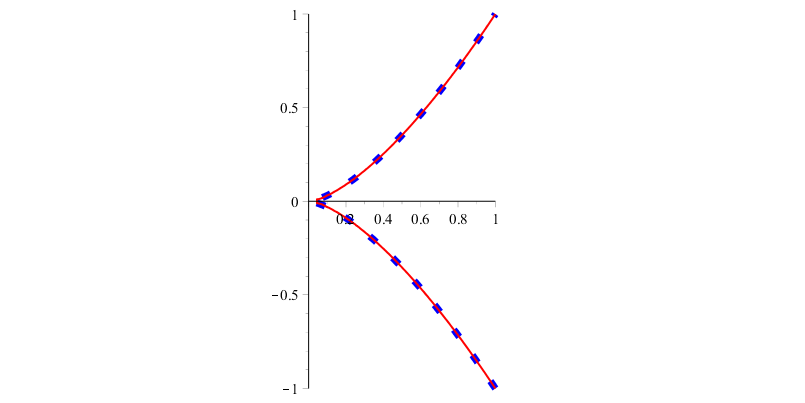
\includegraphics[scale=0.35]{Export/implicitplot1.png}
\end{center}

Vi kan använda Maple för att rita ut både den explicita versionen av kurvan (prickad tjock linje) och den implicita versionen (tunn hel linje). Om vi inte övertygas av den algebraiska representationen, kan den visuella representationen snabbt ge oss en fingervisning hur väl den explicita och den implicita stämmer överens.

\subsection{Exempel --- Lite svårare}
\label{ImplicitNotationEx2}

Låt oss nu studera kurvan $C(t)=(t^2,t^3+t^4)$. Den ser till synes inte mycket svårare ut. Hur ser den implicita formen ut?

\begin{verbatim}
> FindImplicitNotation(t^2, t^3+t^4, t, 30, true);

Elapsed Time: 0.000 s.
\end{verbatim}
\[-x^4+x^3+2x^2y-y^2 = 0\]

Här behövs lite fler operationer genomföras för att $X_p(t)$ och $Y_p(t)$ ska ta ut varandra. I en graf ser de explicita och implicita formerna ut så här:

\begin{center}
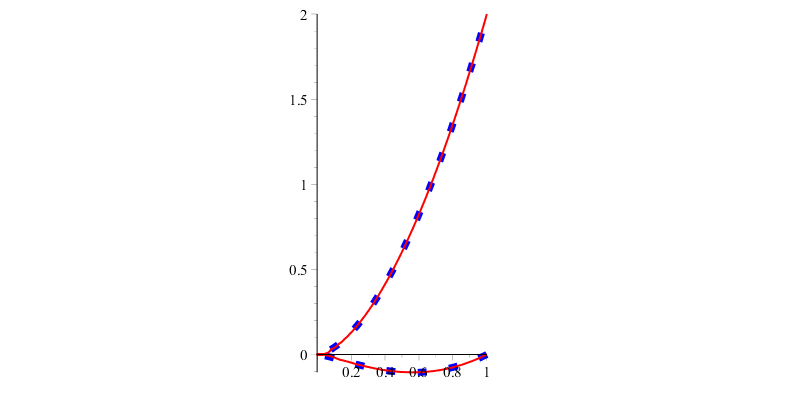
\includegraphics[scale=0.35]{Export/implicitplot2.png}
\end{center}

\subsection{Exempel --- Annan variant på samma}
\label{ImplicitNotationEx3}

Nästa kurva är nästan identisk med föregående. Bara den andra potensen i t-koordinated är lite högre $C(t)=(t^2,t^3+t^7)$.

\begin{verbatim}
> FindImplicitNotation(t^2, t^3+t^7, t, 30, true);

Elapsed Time: 0.000 s.
\end{verbatim}
\[-x^7-2x^5-x^3+y^2 = 0\]

Komplexiteten är samma som föregående kurva. I en graf ser de explicita och implicita formerna ut så här:

\begin{center}
	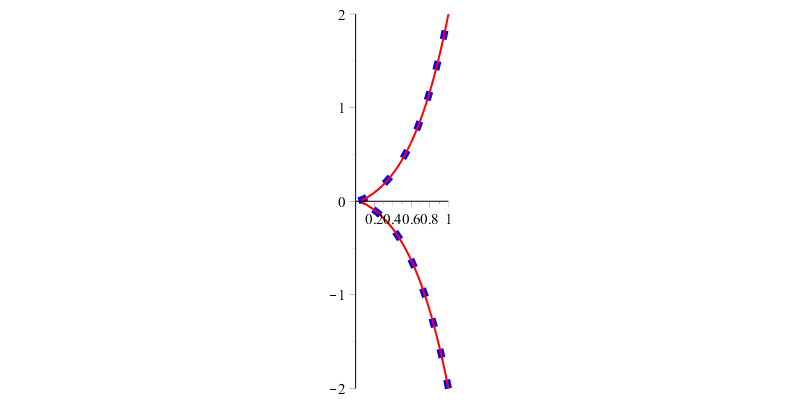
\includegraphics[scale=0.35]{Export/implicitplot3.png}
\end{center}

\subsection{Exempel --- Jmfr. exempel \ref{SimplePolynomialRingExample}}

Detta exempel motsvarar exempel \ref{SimplePolynomialRingExample} till funktionen \emph{FindSemiGroupFromPolynomialRing}: $C(t)=\left(t^2+t^3,t^5+t^6\right)$.

\begin{verbatim}
> FindImplicitNotation(t^4+t^5, t^6+t^7, t, 40, true);

Elapsed Time: 0.000 s.
\end{verbatim}
\[-x^7+2x^4y^2-xy^4+y^5 = 0\]

I en graf ser de explicita och implicita formerna ut så här:

\begin{center}
	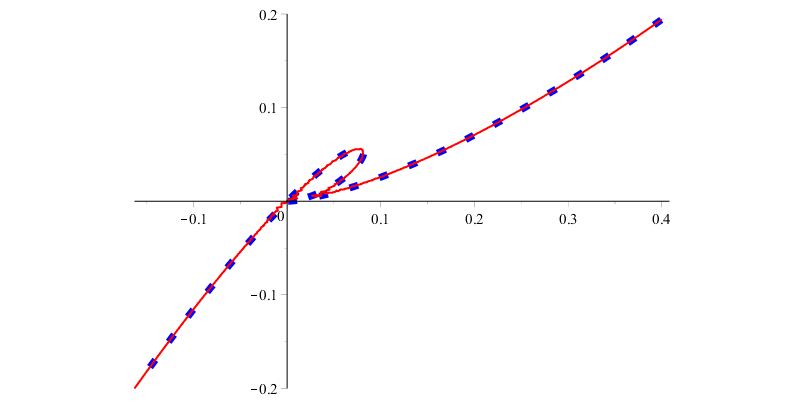
\includegraphics[scale=0.35]{Export/implicitplot4.png}
\end{center}

\subsection{Exempel --- Jmfr. exempel \ref{CostRingExample}}

Detta exempel motsvarar det lite mer beräkningskrävande exemplet \ref{CostRingExample} till funktionen \emph{FindSemiGroupFromPolynomialRing}: $C(t)=\left(t^8+t^{11},t^{12}+t^{13}\right)$.

\begin{verbatim}
> FindImplicitNotation(t^8+t^11, t^12+t^13, t, 150, true);

Elapsed Time: 0.438 s.
\end{verbatim}
\[
\begin{array}{l}
-x^{13}+4x^{10}y^2+5x^9y^3-42x^8y^4-11x^7y^5-6x^7y^4+33x^6y^5-\\
-85x^5y^6+125x^4y^7-14x^3y^8+25x^2y^9+y^{11}+4x^4y^6-25x^3y^7+\\
+36x^2y^8+13xy^9-3y^{10}-xy^8+3y^9 = 0
\end{array}
\]

I en graf ser de explicita och implicita formerna ut så här:

\begin{center}
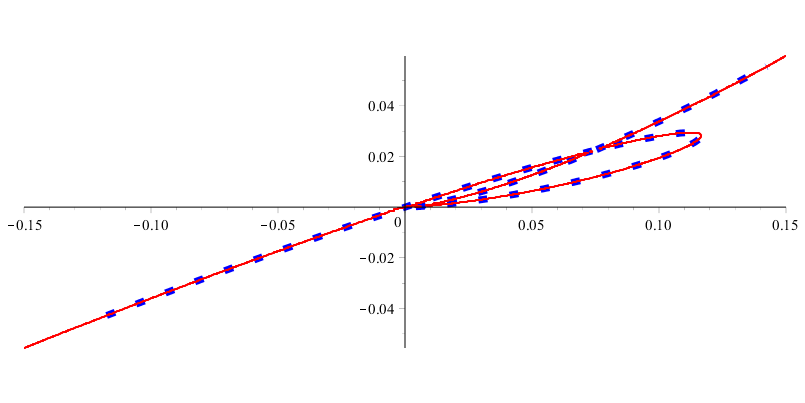
\includegraphics[scale=0.35]{Export/implicitplot5.png}
\end{center}

\subsection{Exempel --- Jmfr. exempel \ref{ReparametrizeSingularities}}

Detta exempel motsvarar rosetten i exemplet \ref{ReparametrizeSingularities} till funktionen \emph{Reparametrize}: $C(t)=\left(t^3(t - 1)^3(t + 1)^3,t^5(t - 1)^2(t + 1)^2\right)$.

\begin{verbatim}
> FindImplicitNotation(t^3*(t-1)^3*(t+1)^3, t^5*(t-1)^2*(t+1)^2, 
     t, 150, true);

Elapsed Time: 1.266 s.
\end{verbatim}
\[
\begin{array}{l}
x^9-9x^8y+36x^7y^2-84x^6y^3+126x^5y^4-126x^4y^5+\\
+84x^3y^6-36x^2y^7+9xy^8-y^9+x^4y^3 = 0
\end{array}
\]

I en graf ser de explicita och implicita formerna ut så här:

\begin{center}
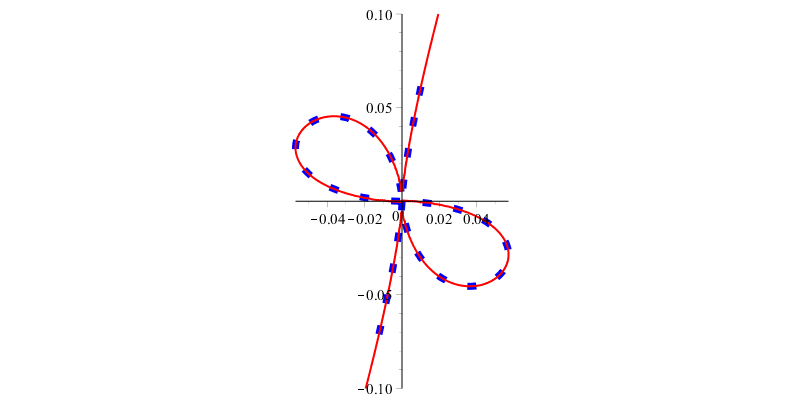
\includegraphics[scale=0.35]{Export/implicitplot6.png}
\end{center}
